\label{sensetivity_results}

One of the attractive characteristics of the Nelder-Mead search algorithm, is its ability to scale to an unlimited number of unknowns.  The main adverse effects of the scaling are the increased number of runs and the combination of the errors.  As the number of unknown increases the complexity of the search space increases, which in turn increases the number of iterations needed to find a minimum.  This can result in drastically longer wait times for the search results.  Additionally, with the increased number of unknowns, the stop condition of the search algorithm will be met at a different interval since the stop condition is based on the variance in the simplex.  This may result in modifications to the stop conditions being necessary as larger number of unknowns are included.  If the response variable is properly defined, it will not affect the models results if more unknowns are included \cite{wang_2011}.

In order to reduce the complexity of the search algorithm, a sensitivity analysis was performed.
This work began by finding the material properties which were needed in the models as summarized in Table \ref{tab:sens_properties}.
\begin{table}[!htb]
	\centering
	\caption{Key material properties in thermal modeling of AM}
	\label{tab:sens_properties}
	\begin{tabular}{|c|c|} \hline
		Material Property & Reference \\ \hline
		Solidus temperature & 
			\begin{tabular}{c}
				\cite{joseph_r_davis_aluminum_2001},
				\cite{lundberg_material_1994},  \\
				\cite{ulbrich_wire_2014},
				\cite{matweb}
			\end{tabular}\\ \hline
		Liquidus temperature & 
			\begin{tabular}{c}
				\cite{joseph_r_davis_aluminum_2001}, 
				\cite{lundberg_material_1994}, \\
				\cite{ulbrich_wire_2014}, 
				\cite{matweb}
			\end{tabular}\\ \hline
		Solid density & 
			\begin{tabular}{c}
				\cite{matweb},
				\cite{amesweb}
			\end{tabular}\\ \hline
		Fluid density & 
			\begin{tabular}{c}
				\cite{matweb},
				\cite{schmitz_density_2012},\\
				\cite{leitner_thermophysical_2017}
			\end{tabular}\\ \hline
		Specific heat & 
			\begin{tabular}{c}
				\cite{lundberg_material_1994},
				\cite{leitner_thermophysical_2017}
			\end{tabular}\\ \hline
		Thermal conductivity & 
			\begin{tabular}{c}
				\cite{lundberg_material_1994},
				\cite{leitner_thermophysical_2017}
			\end{tabular}\\ \hline
		Absorptivity & 
			\begin{tabular}{c}
				\cite{funck_tailored_2014},
				\cite{boyden_temperature_2006},\\
				\cite{el-hameed_anodic_2017}
			\end{tabular}\\ \hline
	\end{tabular}
\end{table}

These properties were varied according to a Placket-Burman design of experiment in order to determine the properties which, when changed, had a statically significant effect on the resulting melt pool width, depth, and volume, as measured in Figure \ref{fig:slices}.
\begin{figure}[!tb]\centering
	\begin{subfigure}[t]{0.22\textwidth}\centering
	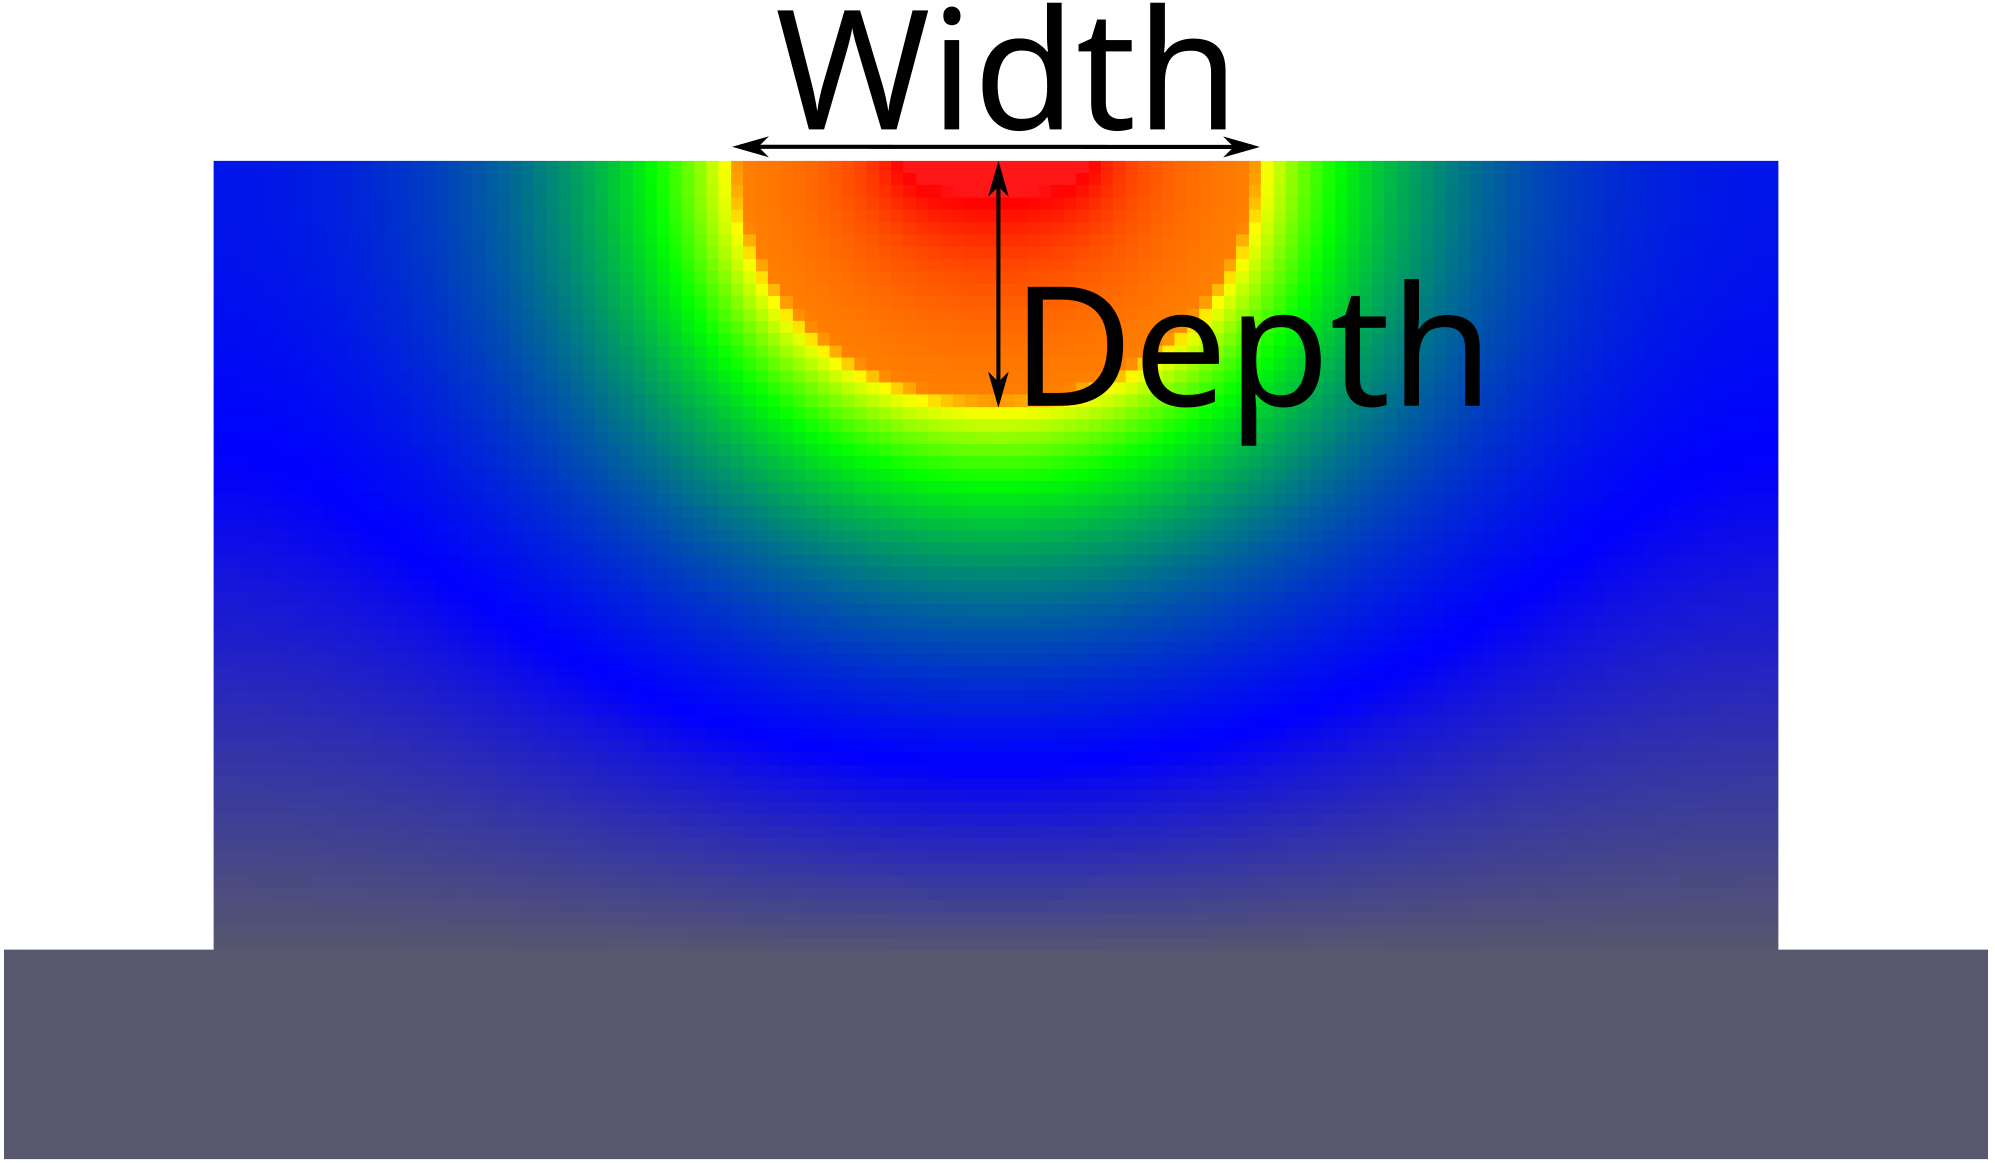
\includegraphics[height=0.6in]{slice_y_annotated}
	\caption{Width}
	\label{fig:slice_y_annotated}
	\end{subfigure}
		\begin{subfigure}[t]{0.77\textwidth}\centering
		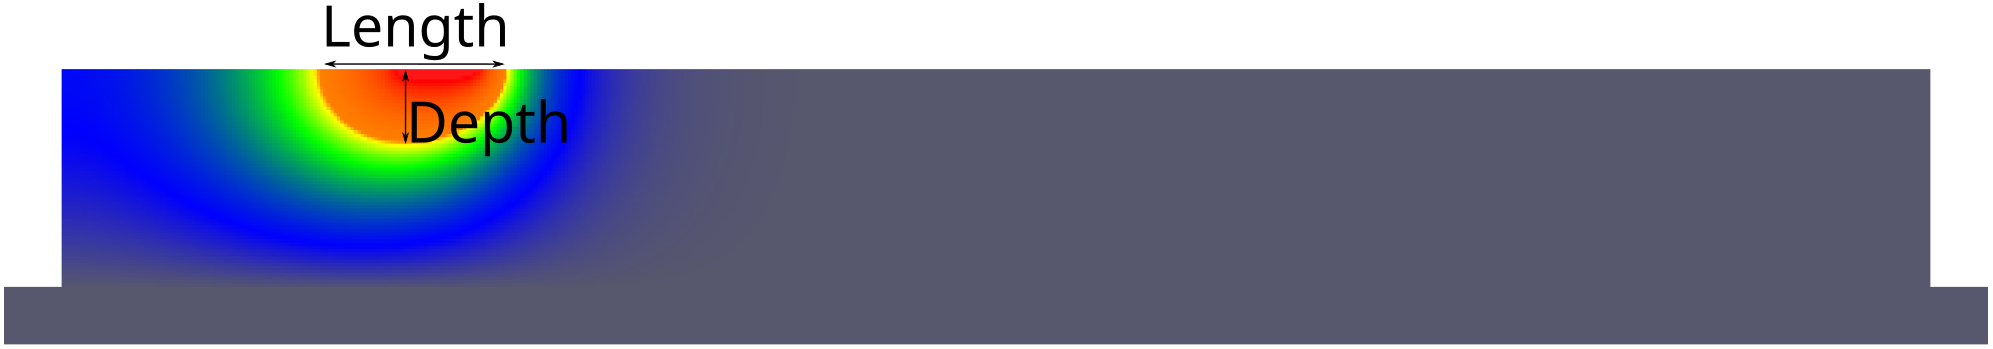
\includegraphics[height=0.6in]{slice_x_annotated}
		\caption{Length}
		\label{fig:slice_x_annotated}
		\end{subfigure}
	\caption{Example measurements of the melt pool}
	\label{fig:slices}
\end{figure}
Analyzing these results with Pareto charts of the standardized effects of the variables and partial regression plots of the residuals it was determined that the variables in Table \ref{tab:crit_mat_prop} had a statically significant effect on the resulting melt track when modified.
\begin{table}[!htb]
	\centering
	\caption{Critical material properties}
	\label{tab:crit_mat_prop}
		\begin{tabular}{|c|} \hline 
			Laser absorption at 880\degree C \\ \hline
			Laser absorption at 922\degree C \\ \hline
			Thermal conductivity at 922\degree C \\ \hline
			Thermal conductivity at 1491\degree C \\ \hline
			Specific heat at 733\degree C \\ \hline
		\end{tabular}
\end{table}
This work included the laser diameter in the search algorithms dataset due to the difficulty associated with accurately measuring the diameter.
